\documentclass{my_paper}
\usepackage{ctex}
\usepackage[textwidth=444bp,vmargin=2.5cm]{geometry}%设置页边距
\usepackage{array} %主要是增加列样式选项
\usepackage[dvipsnames]{xcolor}%颜色宏包
\usepackage{graphicx}%图片宏包
\usepackage{amsmath}%公式宏包
\usepackage[T1]{fontenc}    
\usepackage{newtxtext, newtxmath}  %两种使用Times New Roman 字体的方法
\usepackage{cite}

\begin{document}
%----------- 中文摘要 ----------
\begin{titlepage}

    \begin{center}


        % Upper part of the page
        
\includegraphics[width=0.8\textwidth]{hitlogo.png}\\[1cm]

        \textsc{\LARGE Harbin Institute of Technology}\\[1.5cm]

        % Title
        \hrulefill \\[0.4cm]
        { \huge \bfseries 烤盘形状的最优化分析}\\[0.4cm]
        \hrulefill \\[1.5cm]

        % Author and supervisor
        \begin{minipage}{0.4\textwidth}
            \begin{flushleft} \large
                %悬空
            \end{flushleft}
        \end{minipage}
        \begin{center}
            \large
            \bfseries
            \emph{2021113679 \quad 吴嘉阳}\\
            \emph{2021111975 \quad 涂羽冲}
        \end{center}

        \vfill

        % Bottom of the page
        {\large \today}

    \end{center}
\end{titlepage}


\newpage
\begin{center}
    \zhaiyao
\end{center}

为了充分使用烤箱面积以及最优化烤盘的温度,本文针对烤盘的形状进行研究,主要解决了不同形状烤盘上温度分布的计算问题,考虑了在烤盘个数最对和温度分布均匀性最大的条件下的烤盘形状。

模型1从传热学理论入手,结合烤箱的恒温工作原理进行合理化假设,在热传导的基础上建立了含热对流因素的烤盘传热方程。通过简化并求解其稳态解,得出了烤盘四角过热的原因以及变化规律,同时考虑了热传导和热对流,并将边缘的温度方差条件进行标幺化,构建了针对不同正多边形的评估函数。

模型2在简历过程中,对目标函数的两个指标进行了修正分析,使得两个指标随自自变量的变化速度近似相同,以方便加权优化。并利用整数规划求解出最优长宽比以及p的值。

\begin{guanjianci}
    热传导 \quad 双目标优化 \quad 目标规划 \quad 整数规划
\end{guanjianci}

\vspace{2em}

\tableofcontents

%----------- 正文 ----------
%----------- 一、问题重述 ----------
\newpage
\section{一、问题重述}
随着经济的发展,烤箱进入了人们的日常生活,烘烤食物成为了最普通的需求之一。但是在使用不同烤盘烘烤食物的时候,会出现食物受热不均匀的问题,而烘烤食物个数与烤盘的空间利用率同样也是我们的考虑因素,因此建立烤盘形状的最优化模型有着重要的意义。

在建立数学模型的过程中,为了确定最佳的烤盘形状,我们需要考虑以下因素:

(1)烤盘的均匀受热情况最大化;

(2)烤箱容纳烤盘数量的最大化;

(3)组合以上两种情况,构建双目标优化模型,分别用$p$与$1-p$来表示权重分配,随着烤盘形状与$p$的变化,展示出结果的变化。

在建立优化模型的过程中,分为以下几个步骤:

(1)建立描述不同形状的烤盘的受热均匀程度的量;

(2)选取、确定烤盘摆放的方式;

(3)构建组合优化的评价函数,并求解最优化问题。

\section{二、模型假设}
(1)烤箱内部温度恒定,空气强制对流;

(2)烤箱采用导热性能良好且各项通行的介质制作而成;

(3)烤盘形状近似为无盖的多边形柱体,其中,长方形烤盘的形状大致如图\ref{pan}所示;

(4)烤盘内部没有热源,忽略烤盘厚度。

\begin{figure}[h]
    \centering
    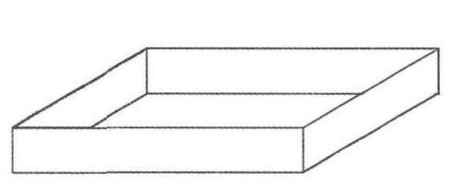
\includegraphics[width=0.5\textwidth]{pan.jpg}
    \caption{烤盘形状基本模型图}
    \label{pan}
\end{figure}

\newpage
%----------- 四、符号说明 ----------
\section{三、符号说明}
%使用三线表格最好~
\begin{table}[h]%htbp表示的意思是latex会尽量满足排在前面的浮动格式,就是h-t-b-p这个顺序,让排版的效果尽量好。
    \centering
    \begin{tabular}{p{2.0cm}<{\centering}p{9.0cm}<{\centering}p{2.0cm}<{\centering}}
        %指定单元格宽度, 并且水平居中。
        \hline
        符号    & 说明       & 单位                 \\ %换行 
        \hline
        $A$     & 烤箱面积   & $m^2$                \\
        $S$     & 烤盘面积   & $m^2$                \\
        $T$     & 温度       & $\circ C$            \\
        $\rho$  & 材料密度   & $kg/m^{3}$           \\
        $Q_{g}$ & 内热源     & $J$                  \\
        $h$     & 热对流系数 & $W/(K \cdot m^{2} )$ \\
        \hline
    \end{tabular}
\end{table}

%----------- 五、模型的建立与求解 ----------
\section{四、模型的建立与求解}

\subsection{热传导模型的建立}
\subsubsection{模型的建立}
根据热力学的基本理论,热传递有三种方式,热传导、热对流和热辐射。在烤箱中,热空气携带的热量通过热对流或风扇强制对流传递给烘焙的食物。这些热量可能来自于箱内空气热对流,也可能来源于烤箱加热表面的热辐射,或者来源于食物与烤箱接触金属部分的热传导过程。\cite{sakin2009convection} 在大部分温度可控的烤箱中由于烤箱中的气体温度可以保持恒定,导致食物边缘烤焦的不均匀热源主要来自金属烤盘。因此本模型着重分析金属烤盘的热传递过程。

构建的金属烤盘的热流的示意图如图\ref{heatflow}所示。
\begin{figure}[h]
    \centering
    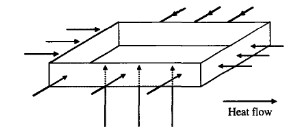
\includegraphics[width=0.5\textwidth]{heatflow.jpg}
    \caption{烤盘热流示意图}
    \label{heatflow}
\end{figure}

基于假设中各向同性条件,恒温箱中烤盘各个面所接收的热流密度相同,因此,烤盘中热分布不均是烤盘与空气之间的热对流和金属烤盘金属材料之间的热传导所造成的。根据热传导方程,
\begin{equation}
    \rho c \frac{\partial T}{\partial t}-\lambda (\frac{\partial^{2} T}{\partial x^{2}}+\frac{\partial^{2} T}{\partial y^{2}}+\frac{\partial^{2} T}{\partial z^{2}})= Q_{g}
    \label{heat_tranfer_equation}
\end{equation}

在热传导过程达到问题的时候,温度不再改变,故
\begin{equation}
    \frac{\partial T}{\partial t}=0,t \to \infty
    \label{temperature}
\end{equation}

该微分方程的边界条件采用诺依曼边界条件(Neumann foundary condition),即已知各面的法向热流密度$q_{edge}:q_{edge}=-\lambda \frac{\partial T}{\partial n}=q(x,y,z,t)$,其中$\vec{n}$为外法线方向。


由式\ref{temperature}可以得到含有热对流因素、无热源的稳态热传递方程,即烤盘的稳态热传递方程

\begin{equation}
    -\lambda(\frac{\partial^{2} T}{\partial x^{2}}+\frac{\partial^{2} T}{\partial y^{2}}+\frac{\partial^{2} T}{\partial z^{2}})=h(T_{ext}-T)
    \label{pan_heat_transfer_equation}
\end{equation}

如果仅考虑烤盘底面受热,忽略烤盘侧面,则烤盘表面的热分布将会平均。因此烤盘热分布不均是侧面接收的热量向底面传到造成的,故可将三围的热传递模型近似简化为二维平面热传递模型。

\begin{equation}
    \left\{
    \begin{aligned}
         & -\lambda(\frac{\partial^{2} T}{\partial x^{2}}+\frac{\partial^{2} T}{\partial y^{2}}+\frac{\partial^{2} T}{\partial z^{2}})=h(T_{ext}-T) \\
         & q_{edge}=-\lambda \frac{\partial T}{\partial \vec{n}}=q_{0}
    \end{aligned}
    \right.
    \label{heat_tranfer_function}
\end{equation}



\subsubsection{模型的求解}

利用$Matlab$提供的PDEtool工具计算,可得到二维热传递模型的数值解。\cite{burstein2022pde}其中烤盘的各项参数以及边界条件如表所示。

\begin{table}[h]%htbp表示的意思是latex会尽量满足排在前面的浮动格式,就是h-t-b-p这个顺序,让排版的效果尽量好。
    \centering
    \caption{标准状态下各项参数设置}
    \begin{tabular}{p{2.0cm}<{\centering}p{9.0cm}<{\centering}p{2.0cm}<{\centering}}
        %指定单元格宽度, 并且水平居中。
        \hline
        物理量    & 参数值                   \\
        \hline
        $\lambda$ & $50/(W/(K\cdot m))$      \\
        $h$       & $100/(W/(K\cdot m_{2}))$ \\
        $T_{ext}$ & $330/K$                  \\
        $q_{0}$   & $1000/(W/(s\cdot m))$    \\
        \hline
    \end{tabular}
\end{table}


得到温度标准差代表边缘的热平均度,如表\ref{temperature_variance}所示\cite{songyankan}。


\begin{table}[h]
    \centering
    \caption{标准状态下各项参数设置}

    \begin{tabular}{p{2.0cm}<{\centering}p{9.0cm}<{\centering}p{2.0cm}<{\centering}}
        %指定单元格宽度, 并且水平居中。
        \hline
        正多边形边数 & 边缘温度标准差($\sigma_{m}$) & 标幺值 \\
        \hline
        4            & 1.5139                       & 1      \\
        5            & 0.8342                       & 0.5510 \\
        6            & 0.5845                       & 0.3861 \\
        7            & 0.4142                       & 0.2736 \\
        8            & 0.3100                       & 0.2048 \\
        10           & 0.2313                       & 0.1528 \\
        14           & 0.0948                       & 0.0627 \\
        16           & 0.0755                       & 0.0499 \\
        $\infty$     & 0.0000                       & 0      \\

        \hline
    \end{tabular}
    \label{temperature_variance}
\end{table}


从表\ref{temperature_variance}可以看出,随着多边形边数的增多,整体温度方差和边缘方差均逐渐减小。同时,随着多边形数增多,整体温度方差趋近于一个恒定值,边缘温度方差趋于0。边缘性状决定边缘热分布,同时影响着整体热分布的平均程度。边数越多,边缘越光滑,整体热分布越平均。因此,可用边缘热分布的标准差来衡量烤盘热分布的均匀程度。

利用Matlab拟合,可得利用标准差表示的热平均度与正多边形$m$近似存在关系:
\begin{equation}
    \sigma=\frac{23.606}{m^{2}}+0.025\approx \frac{23.605}{m^2}\propto \frac{1}{m^{2}}
    \label{heat_variance}
\end{equation}

本模型及其结果合理地解释了长方形烤盘边缘受热不均匀的问题,同时揭示了烤盘形状由多边形向圆形逼近时,边缘热分布逐渐平均的变化规律。


\subsection{最优化烤盘设计}

根据模型一以及对题目的分析研究可以知道,热分布的均匀程度随着烤盘性状的变化而变化。为了优化烤盘,需要考虑烤盘面积剩余率与温度差异程度。

\subsubsection{烤盘面积剩余率$\eta$}
定义烤盘面积剩余率:$\eta = 1-\frac{NA}{2S}$,其中:$A$表示单个烤盘面积,$N$表示烤架上烤盘总数量,$S$表示烤架的面积。$eta$越小,烤盘面积利用率越高。

根据平面镶嵌原理,正多边形中只有矩形(含正方形)、正六边形可以无间隙且不重叠地覆盖无限大的平面,其他图形(包括圆)都无法做到无间隙覆盖。因此,只有使用矩形、挣了六边形烤盘才可使烤架面积利用率饱和。而对于有限平面,由于存在边界形状限制,有存在边界约束,情况较为复杂。

\subsubsection{烤盘温度差异程度$\sigma$}
在模型一中讨论了利用边缘温度标准差来衡量烤盘热分布均匀程度的可行性。在此,定义烤盘温度差异程度$\sigma=\frac{\sum n_{i} \sigma_{i}}{\sigma_{0}N}$,其中:$\sigma_{i}$为第$i$中烤盘的边缘温度差;$n_{i}$为第$i$种烤盘的数量。为方便后续组合优化分析,在此公式中将方差标幺化,使之成为无量纲量,取烤盘为正方形时,最大标准差$\sigma_{0}$为标准值,$\sigma$越小表明烤盘各部分温度差异性越小,热分布越均匀。

根据模型一的结论,正多边形边缘的热分布平均程度与其边数的平方成反比,故圆形烤盘的热均匀度最高,而矩形的热均匀度最低。若仅考虑热分布均匀程度,完全采用圆形烤盘分布的时候,烤盘温度差异程度最低。

根据不同用户对烤盘需求的不同,设定$p$为烤盘面积剩余率的权重,$(1-p)$为烤盘温度差异程度$\sigma$的权重。需求指定与目标方向为
\begin{equation}
    min[R\cdot \eta p+\sigma(1-p)]
\end{equation}
其中,$R$为修正因子,用来修正形状变化过程中两种因素的变化速度,使两种因素的变化速度尽可能相似,以使优化更准确。

基本约束条件如下
\begin{equation}
    s.t.\left\{
    \begin{aligned}
         & 2S-NA \ge 0                  \\
         & \sum n_{i}=N,n_{i} \in Z_{+}
    \end{aligned}
    \right.
\end{equation}

\subsubsection{目标函数的最优化问题}
为了解决双目标优化问题,我们限定$0<p<1$,这样既能使烤盘的受热分布均匀,减小事物边角烤焦的奉献,也能充分利用烤盘。

对于任何4l面体,在采取边与边重叠排布时,其包围的空隙图形为$4(l-1)$面体,其空隙面积与边数的关系为
\begin{equation*}
    S_{l}=A(\frac{\cot \frac{\pi}{4l}}{l}-1)
\end{equation*}
该函数随$l$的变化速度与$\sigma$的变化速度近似相同,方向相反,因此$R$应该取常数。我们仅考虑矩形、正六边形、正八边形、圆形的情况。

\paragraph{测试1}:$p=0.5,W/L=9/13=0.6923,N=40,m=6,a=3.3981cm$,结果如图\ref{test1}所示。此时,目标函数取极小值,即:
\begin{equation*}
    f(p=0.5)_{min}=0.5(1-\frac{40\times 30}{2\times 754.8372})+0.5 \times 0.3861=0.2956
\end{equation*}

\begin{figure}[h]
    \centering
    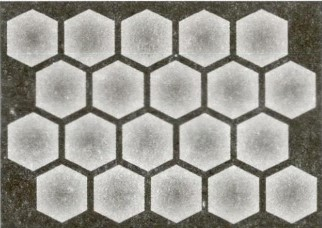
\includegraphics[width=0.5\textwidth]{test1.jpg}
    \caption{测试1的最优排布图}
    \label{test1}
\end{figure}


\paragraph{测试2}:$p=0.25,W/L=9/13=0.6923,N=30,m=8,a=2.4926cm$,结果如图\ref{test2}所示。此时,目标函数取极小值,即:
\begin{equation*}
    f(p=0.25)_{min}=0.25(1-\frac{30\times 30}{2\times 754.8372})+0.75 \times 0.2048=0.2546
\end{equation*}


\paragraph{测试3}:$p=0.5,W/L=0.6833,N=30,m=8,a=2.4926cm$,结果如图\ref{test1}所示。此时,目标函数取极小值,即:
\begin{equation*}
    f(p=0.5)_{min}=0.5(1-\frac{40\times 30}{2\times 754.8372})+0.5 \times 0.2048=0.2050
\end{equation*}

\begin{figure}[htbp]
    \centering
    \begin{minipage}[t]{0.48\textwidth}
        \centering
        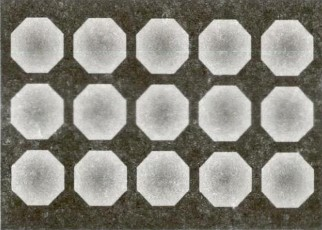
\includegraphics[width=6cm]{test2.jpg}
        \caption{测试2的最优排布图}
        \label{test2}
    \end{minipage}
    \begin{minipage}[t]{0.48\textwidth}
        \centering
        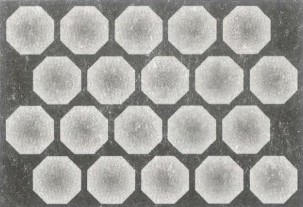
\includegraphics[width=6cm]{test3.jpg}
        \caption{测试3的最优排布图}
        \label{test3}
    \end{minipage}
\end{figure}

由以上三种情况可以看出,当长宽比不变时,权重p的变化使最优解和排布方式发生了变化;当p不变,$W/L$改变时,最优解和排布方式也发生了变化。


%----------- 六、模型的分析与检验 ----------
\section{五、模型的分析与检验}
本问题的优化模型是整数规划模型,因而其随着参数$p$和$W/L$变化呈现的最优解存在离散化的特性。这种特性的存在,使得烤盘种类数量有限化,大大降低了设计成本,使工业生产成为可能,同时由于存在用户需求权重$p$,使得烤盘中类多样化,满足了用户需求。

然而由于这种离散化的特性,使最优解在随着某些量值(如$W/L$)变化时会出现突变。因此在设计烤盘的长宽比时应该尽量在边界点附近多次取指,或者避开边界点,一面造成优化错误。

\section{六、模型的评价、改进与推广}

\subsection{模型的优点}
模型1从传热学理论入手,结合烤箱的恒温工作原理进行合理化假设,在热传导的基础上建立了含热对流因素的烤盘传热方程。通过简化并求解其稳态解,得出了烤盘四角过热的原因以及变化规律,同时考虑了热传导和热对流,使结果更具有说服力。

模型2在简历过程中,对目标函数的两个指标进行了修正分析,使得两个指标随自自变量的变化速度近似相同,以方便加权优化。

\subsection{模型的改进}
模型还可以考虑在圆角矩形条件下的最优化问题,在工业生产中,倒角工艺也是常用的容易实现的方法。





\bibliographystyle{unsrt} 
\bibliography{refs}


\end{document}